% =========================================================
% SUBIR ESTE CÓDIGO COMO CAPÍTULO DE PRÁCTICA EN LA MEMORIA
% =========================================================
\chapter{Cuaderno de Laboratorio — Práctica 3: Metodología de Evaluación y Rigor Científico}

\section*{Objetivo}
Aprender a realizar evaluaciones honestas en condiciones difíciles, especialmente con datos desbalanceados,
y detectar errores metodológicos graves como la fuga de datos (\textit{data leakage}).

\section*{Material de partida}
Se parte de:
\begin{itemize}
    \item Un dataset sintético de \textbf{1000 pacientes} con \textbf{5 variables predictoras}.
    \item Una clase positiva muy minoritaria (\textbf{2\%} de los casos).
\end{itemize}

\section{Tarea 1 — La lotería de la partición aleatoria}

\subsection*{Configuración común}
Modelo usado: \underline{\hspace{6cm}}\\
Métricas usadas: \underline{\hspace{5cm}}\\
Semilla(s): \underline{\hspace{8cm}}

\vspace{0.3cm}
\noindent\textbf{Hipótesis inicial (antes de ejecutar):}
¿Crees que el número de positivos en test será estable? ¿Por qué?
\vspace{1.2cm}

\subsection{Registro de resultados (5 particiones aleatorias)}
\begin{center}
\begin{tabular}{|c|c|}
\hline
Ejecución & Positivos en test \\
\hline
1 & \underline{\hspace{2.5cm}} \\
2 & \underline{\hspace{2.5cm}} \\
3 & \underline{\hspace{2.5cm}} \\
4 & \underline{\hspace{2.5cm}} \\
5 & \underline{\hspace{2.5cm}} \\
\hline
\end{tabular}
\end{center}

\begin{center}
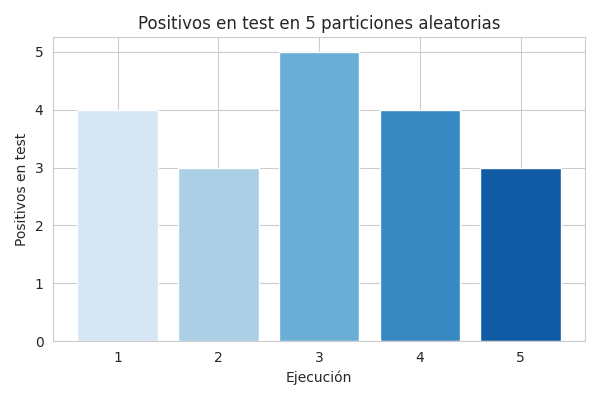
\includegraphics[width=0.85\linewidth]{outputs/tarea1_positivos_test_aleatorio.png}
\end{center}

\noindent\textbf{Análisis:}
\begin{itemize}
    \item ¿Ha cambiado mucho el número de positivos en test entre ejecuciones?
    \item ¿Sería fiable la evaluación si el azar dejara solo 0 o 1 positivos en test?
\end{itemize}

\vspace{1.5cm}

\section{Tarea 2 — Partición estratificada}

\subsection{Registro por folds}
\begin{center}
\begin{tabular}{|c|c|c|c|}
\hline
Fold & Positivos en test & Tamaño del fold & Proporción clase 1 \\
\hline
1 & \underline{\hspace{1.8cm}} & \underline{\hspace{1.8cm}} & \underline{\hspace{2.0cm}} \\
2 & \underline{\hspace{1.8cm}} & \underline{\hspace{1.8cm}} & \underline{\hspace{2.0cm}} \\
3 & \underline{\hspace{1.8cm}} & \underline{\hspace{1.8cm}} & \underline{\hspace{2.0cm}} \\
4 & \underline{\hspace{1.8cm}} & \underline{\hspace{1.8cm}} & \underline{\hspace{2.0cm}} \\
5 & \underline{\hspace{1.8cm}} & \underline{\hspace{1.8cm}} & \underline{\hspace{2.0cm}} \\
\hline
\end{tabular}
\end{center}

\begin{center}
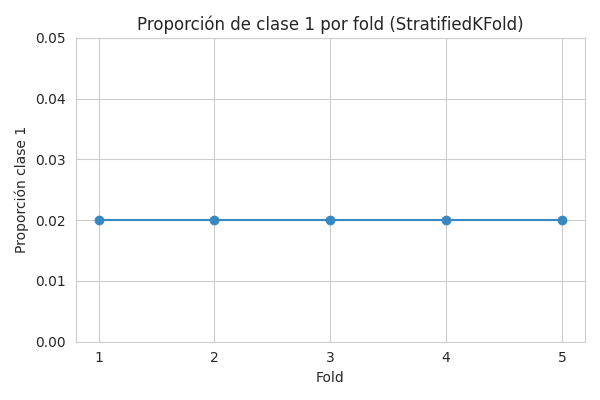
\includegraphics[width=0.85\linewidth]{outputs/tarea2_proporcion_folds_estratificado.png}
\end{center}

\noindent\textbf{Análisis:}
Explica por qué \texttt{StratifiedKFold} es más adecuado que una partición aleatoria simple en este problema.
\vspace{1.6cm}

\section{Tarea 3 — Comparativa de la varianza}

\subsection{Resumen de resultados}
\begin{center}
\begin{tabular}{|c|c|c|c|c|}
\hline
Método & Accuracy media & std(Accuracy) & F1 media & std(F1) \\
\hline
KFold & 0.991 & 0.016 & 0.800 & 0.310 \\
StratifiedKFold & 0.997 & 0.002 & 0.914 & 0.070 \\
\hline
\end{tabular}
\end{center}

\begin{figure}[H]
    \centering
    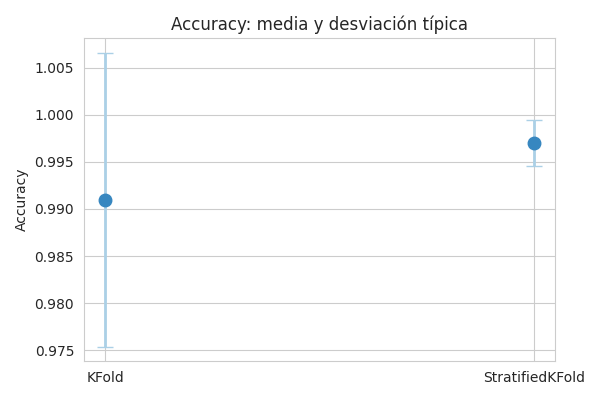
\includegraphics[width=0.85\linewidth]{outputs/tarea3_accuracy_errorpoints.png}
    \caption{Accuracy: media y desviación típica para KFold y StratifiedKFold.}
    \label{fig:t3_accuracy}
\end{figure}

\begin{figure}[H]
    \centering
    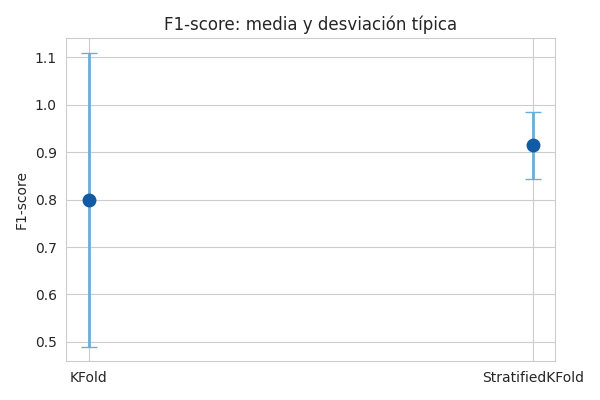
\includegraphics[width=0.85\linewidth]{outputs/tarea3_f1_errorpoints.png}
    \caption{F1-score: media y desviación típica para KFold y StratifiedKFold.}
    \label{fig:t3_f1}
\end{figure}

\begin{figure}[H]
    \centering
    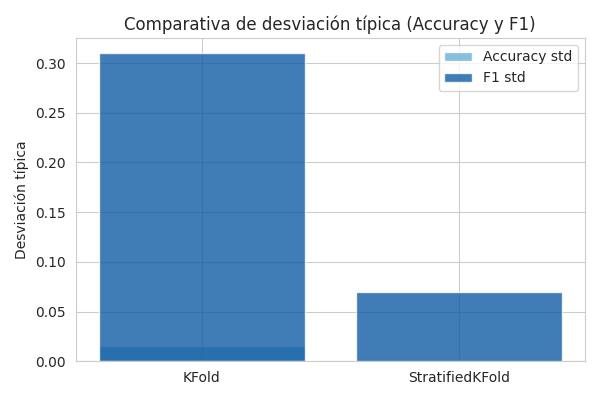
\includegraphics[width=0.85\linewidth]{outputs/tarea3_std_barras.png}
    \caption{Comparativa de desviación típica en Accuracy y F1 entre ambos métodos.}
    \label{fig:t3_std}
\end{figure}

\vspace{0.6cm}

\noindent\textbf{Interpretación:}

Las tres gráficas que hemos generado permiten ver de forma muy clara la diferencia de estabilidad entre KFold y StratifiedKFold. En un problema desbalanceado, una partición aleatoria puede generar folds con muy pocos ejemplos de la clase positiva, lo que hace que las métricas cambien mucho de una ejecución a otra. Cuando se mantiene la proporción de clases en cada fold, esta variabilidad desaparece casi por completo. Por eso, el método que produce métricas más estables es \textbf{StratifiedKFold}.

En la gráfica de Accuracy (Figura~\ref{fig:t3_accuracy}) se aprecia que ambos métodos alcanzan valores altos, pero la dispersión de KFold es mayor. Esto indica que el rendimiento de KFold cambia según cómo se repartan los datos en cada fold. Aunque la diferencia en Accuracy no es muy grande, sí se nota que este método depende más del azar y que sus resultados son menos estables.

En la gráfica del F1-score (Figura~\ref{fig:t3_f1}) la diferencia entre ambos métodos se aprecia todavía mejor. El F1 es una métrica muy sensible a cómo se reparten las clases, y por eso cualquier desequilibrio en los folds afecta mucho a su valor. En KFold se observa una variabilidad muy grande: en algunas ejecuciones el modelo detecta bien la clase positiva, y en otras prácticamente no la detecta. En cambio, StratifiedKFold mantiene valores de F1 más altos y, sobre todo, mucho más estables. Esto indica que la estratificación ofrece una evaluación más fiable y refleja mejor el comportamiento real del modelo.

La gráfica comparativa de desviaciones típicas (Figura~\ref{fig:t3_std}) resume perfectamente esta idea: StratifiedKFold reduce la varianza tanto en Accuracy como en F1, pero la mejora es especialmente evidente en F1. Esto tiene sentido, porque F1 es la métrica que más sufre cuando la clase positiva aparece de forma irregular en los folds. Por tanto, \textbf{la mejora se nota mucho más en F1 que en Accuracy}.

En resumen, las gráficas muestran que controlar la proporción de clases en cada fold no cambia el modelo, pero sí cambia la calidad de la evaluación, haciéndola más estable, más fiable y menos dependiente del azar.

\vspace{0.2cm}

\section{Tarea 4 — Detección de data leakage}

\subsection{Comparativa}
\begin{center}
\begin{tabular}{|c|c|c|}
\hline
Escenario & Accuracy & F1 \\
\hline
Sin variable trampa & \underline{\hspace{2cm}} & \underline{\hspace{2cm}} \\
Con variable trampa & \underline{\hspace{2cm}} & \underline{\hspace{2cm}} \\
\hline
\end{tabular}
\end{center}

\begin{center}
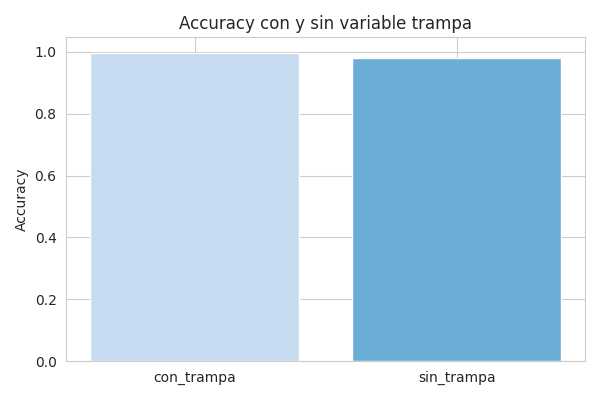
\includegraphics[width=0.85\linewidth]{outputs/tarea4_accuracy_leakage.png}
\end{center}

\begin{center}
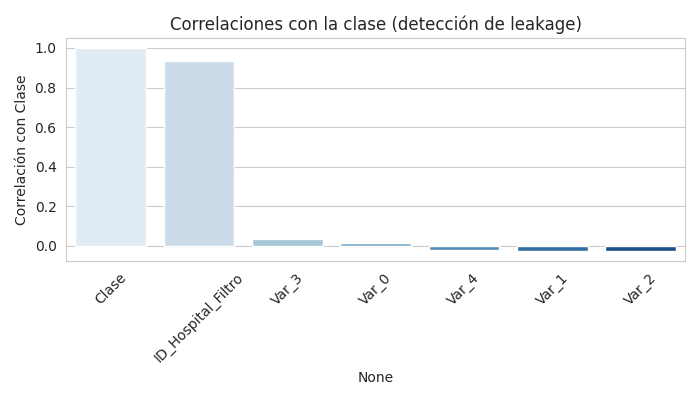
\includegraphics[width=0.90\linewidth]{outputs/tarea4_correlaciones_leakage.png}
\end{center}

\noindent\textbf{Preguntas:}
\begin{itemize}
    \item ¿Qué variable sospechas que está filtrando información del objetivo?
    \item ¿Por qué esa variable invalida la evaluación?
    \item ¿Qué diferencia conceptual hay entre un modelo ``bueno'' y un modelo contaminado por leakage?
\end{itemize}

\vspace{1.4cm}

\section{Reto — Auditoría metodológica}
Redacta un pequeño informe (6--10 líneas) respondiendo a estas cuestiones:
\begin{enumerate}
    \item ¿Por qué una partición aleatoria simple puede ser peligrosa en problemas desbalanceados?
    \item ¿Qué aporta la validación estratificada?
    \item ¿Por qué el \textit{data leakage} puede hacer inútiles las conclusiones de un experimento?
    \item ¿Qué buenas prácticas metodológicas seguirías en futuros experimentos?
\end{enumerate}

\vspace{2cm}

\section{Conclusión final}
Resume qué has aprendido sobre evaluación rigurosa, estabilidad de métricas y detección de errores metodológicos.
